\chapter{Wave Propagation in a Medium}\label{lec:lec26}
In the previous chapter, we discussed Wave Propagation in a medium with finite conductivity.

In this Chapter, we are going to be investigating the wave propagation in a medium that is a good conductor. (i.e. $\sigma \gg \omega$ $\epsilon_{o}$ $\epsilon_{r}$, and the conduction current is much or far larger compared to the displacement current).

Recall,
\begin{center}
$\beta=\omega\sqrt{\dfrac{\mu_{o}\epsilon_{o}\epsilon_{r}}{2}}\Bigg\{{\sqrt{1+\dfrac{\sigma^{2}}{\omega^{2}\epsilon_{o}^{2}\epsilon_{r}^{2}}}+1 }\Bigg\}^{1/2}$
\end{center}

\begin{center}
$\alpha=\omega\sqrt{\dfrac{\mu_{o}\epsilon_{o}\epsilon_{r}}{2}}\Bigg\{\sqrt{1+\dfrac{\sigma^{2}}{\omega^{2}\epsilon_{o}^{2}\epsilon_{r}^{2}}}  -1\Bigg\}^{1/2}$	
\end{center}

This is what we saw earlier, but we want to take a different approach to the problem in a simpler way.
\begin{equation}
\gamma=j\omega\sqrt{\mu\epsilon_{o}}\Bigg\{\sqrt{\epsilon_{r}-j\dfrac{\sigma}{\omega\epsilon_{o}}}\Bigg\}
\end{equation}		
Taking the square of both sides,
$j^{2}= -1$\\ 
and $\gamma^{2}=-\omega^{2}\mu\epsilon_{o}\Bigg\{\epsilon_{r}-j\dfrac{\sigma}{\omega\epsilon_{o}}\Bigg\}$\\
multiplying the numerator and denominator of the RHS  by $j\omega\epsilon_{o}$

$\gamma^{2}=\dfrac{-\omega^{2}\mu\epsilon_{o}}{j\omega\epsilon_{o}}\cdot j\omega\epsilon_{o}\Bigg\{\epsilon_{r}-j\dfrac{\sigma}{\omega\epsilon_{o}}\Bigg\}$

\begin{center}
$\gamma^{2}=-\{-j\}\omega\mu\cdot\{j\omega\epsilon_{o}\epsilon_{r}-j^{2}\sigma\}$
\end{center}

\begin{center}
$\gamma^{2}=j\omega\mu\epsilon_{o}\{\sigma+j\omega\epsilon_{o}\epsilon_{r}\}$	
\end{center}

\begin{center}
$\gamma=\sqrt{j\omega\mu\{\sigma+j\omega\epsilon_{o}\epsilon{r}\}}$	
\end{center}

But if, 
\begin{center}
$\sigma\gg\omega\epsilon_{o}\epsilon{r}$
\end{center}

Then

$\gamma\approx\sqrt{j\omega\mu\sigma}$

Recall from De Moivre's Theorem;	

\begin{center}
$\sqrt{j}=\sqrt{e^{j\frac{\pi}{2}}}=e^{j\frac{\pi}{4}}=\dfrac{1}{\sqrt{2}}+j\dfrac{1}{\sqrt{2}}$
\end{center}

Therefore,

\begin{center}		
$\gamma = \sqrt{\omega\mu\sigma}\{\dfrac{1}{\sqrt{2}}+j\dfrac{1}{\sqrt{2}}\}$

\end{center}

Then we can deduce from the above equation that:

\begin{center}

$\alpha=\sqrt{\dfrac{\omega\mu\sigma}{2}}\hspace{0.15cm}$ and $\hspace{0.15cm}\beta=\sqrt{\dfrac{\omega\mu\sigma}{2}}$

\end{center}

Therefore,
$\alpha\approx\beta$

This means that for this medium, the attenuation constant $\alpha$ and phase constant $\beta$ are almost equal.

If we recall earlier, we had established that the Transmission line is characterized as a Lossy line whenever we had the Phase constant comparable to the Attenuation constant. And we happen to have a similar situation in the wave propagation through a medium that is a good conductor as shown above. We can therefore say that for a good conductor, the medium is like a very lossy transmission line since the attenuation constant is equal to the phase constant.

This means that when the Wave propagates in this medium, the amplitude dies down very rapidly in the direction of propagation. So when the wave tries to enter the conducting medium, Its amplitude reduces very rapidly, since $\alpha=\beta$. So a good conductor is visualized as an extremely lossy transmission line.

However, there is a difference between a Lossy Transmission Line and a good conducting medium. In a lossy line, the power gets lost in the ohmic resistance of the line. So there is a loss of power when the wave is propagated along the Transmission line, but in the case of a good conducting medium, when the wave is attenuating, the power is not necessarily getting lost in the conductor. There is even no power loss when the thickness is small and consequently, we are going to look at the case of $\alpha=\infty$, over zero distance, the wave dies down as it tries to penetrate this medium.

So in the good conducting medium, the wave cannot penetrate the medium because $\alpha$ is very large due to large attenuation. This does not mean that the power is getting lost in the heating medium. Something else is happening, which we are not going to discuss now. However at this point, we can assume that a good conductor is like a lossy transmission line, and that is the reason we can have the quantity $\alpha=\beta$ and the new amplitude will vary as $e^{-\alpha x}$. So if we plot the wave amplitude as a function of x when we travel a distance $x=\frac{1}{\alpha}$, the wave amplitude will die down to $\frac{1}{e}$ of its initial value.
\begin{figure}[h]
\centering
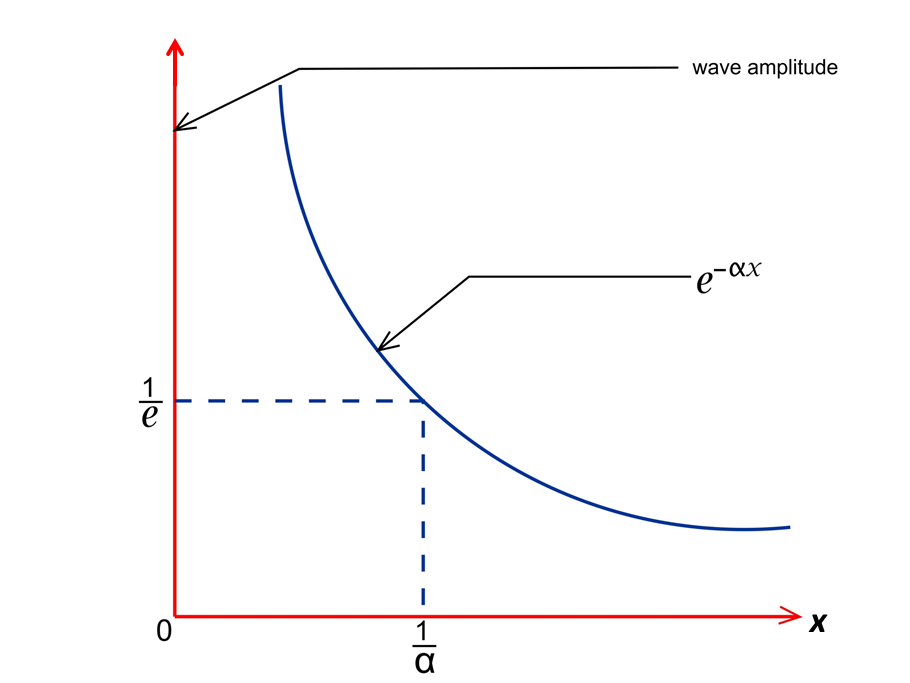
\includegraphics[width=0.9\linewidth]{\pathtopartone/graphics/wave_amplitude_as_function_of_x}
\caption{Wave amplitude as a function of x}
\label{fig:bello261}
\end{figure}

So we can say that when the wave tries to propagate in this conducting medium effectively, the propagation of the wave is over the distance $\frac{1}{\alpha}$, as beyond $\frac{1}{\alpha}$ distance the field is very small. As a rule of thumb, we can say that the wave will propagate over a distance of $\frac{1}{\alpha}$ into the medium. This is the effective length over which the propagation of the wave takes place from the beginning of the medium. We can therefore say that any electromagnetic wave cannot go deep into a conducting medium. It penetrates a little bit from the surface of the conductor. i.e. if the energy in an electromagnetic wave tries to go into a conducting medium, it goes only a short distance from the surface of the conducting medium, and deeper into the conducting medium, the fields are extremely small. This creates a surface phenomenon on the surface of the conductor. So if $\frac{1}{\alpha}$  is the effective length over which the wave propagates, we can say that beyond $\frac{1}{\alpha}$, the field does not exist, so only $\frac{1}{\alpha}$ thickness of the conductor will matter in the conduction of electromagnetic waves. Beyond $\frac{1}{\alpha}$  the field is assumed to be too small and can be neglected. Hence only $\frac{1}{\alpha}$ of the thickness of the conducting medium is what will decide the propagation characteristics of the electromagnetic wave. Deeper in the conducting medium is of no relevance as the field dies down rapidly as you go inside the conducting medium.

\section{\textbf{Effective Depth}}

Effective depth is always represented by $\delta$ and it is given by:
\[
\delta=\frac{1}{\alpha}
\]

Recall,
\begin{center}
$\alpha=\sqrt{\dfrac{\omega\mu\sigma}{2}}$
\end{center}

Therefore,
\begin{center}
$\delta=\dfrac{1}{\sqrt{\frac{\omega\mu\sigma}{2}}}=\sqrt{\dfrac{2}{\omega\mu\sigma}}$
\end{center}

And $\omega=2\pi f$,
\begin{center}
$\delta=\sqrt{\dfrac{2}{2\pi f\mu\sigma}}=\sqrt{\dfrac{1}{\pi f \mu\sigma}}$	
\end{center}

Effective Depth, \begin{center}
$\delta=\sqrt{\dfrac{1}{\pi f \mu\sigma}}$
\end{center}

This can be seen to be inversely related to $\sqrt{f}$,$\sqrt{\mu}$, and $\sqrt{{\sigma}}$, therefore, when there is an increase in frequency or $\sigma$, the depth of penetration of the electromagnetic wave into the conducting medium decreases. With $\sigma=\infty$(i.e. Ideal Conductor), $\delta=0$, that is the wave will not penetrate the medium at all. Similarly, if we go into very high arbitrary frequencies, the depth of penetration becomes extremely small. Let's take typical numbers just to get a feel for what depth we have when we operate at low frequencies.

Let us take an arbitrary medium of conductivity $\sigma=10^{7}\Omega^{-1}m^{-1}$(this is the typical value for a good conductor), $f=100Mhz$(typical value for radio transmission).

Recall,

$\delta=\sqrt{\dfrac{1}{\pi f\mu\sigma}}=\sqrt{\dfrac{1}{\pi\times 100\times 10^{6}\times 4\pi\times 10^{-7}\times 10^{7}}}=1.6\times 10^{-5}m=16\mu m$
\\
So, for a medium that is a good conductor with the conductivity of the order of  $ 10^{7}\Omega^{-1}m^{-1} $ (copper has $ 5.6 \times 10^{7}\Omega^{-1}m^{-1} $), like copper or silver and a frequency of 100MHz to propagate our electromagnetic wave, It will not go deeper than $16\mu m$ from its surface. So if we go to frequencies of GHz used for satellites or microwave frequencies, the effective depth becomes even smaller. So effectively, for a good conductor, if we take a frequency which is a typical radio frequency, the depth of penetration is of few microns to tens of microns. So basically, this propagation is taking place on the skin of the material of the order of a few tens of microns. This is the reason we call this effective depth the \textbf{SKIN DEPTH OF THE MATERIAL}.

Skin Depth is a parameter that tells how electromagnetic energy is going to exist on a good conducting material or medium. Beyond this depth, the propagation does not matter as the field would have died out. So if you have a high-frequency component, since the energy is going to lie on the surface at a few microns or tens of microns, we have to make that layer very good, because any perturbation in the properties of that layer will affect the propagation of the electromagnetic wave. So if we have a conductor and want to send some high-frequency signal through this conductor, the field is essentially going to lie only on the surface of the conductor in the skin depth.

The current excited in this conductor will essentially be confined to the skin depth of the conductor. That is the region in which the field is going to exist and the current will flow in that skin depth.
\begin{figure}[h]
\centering
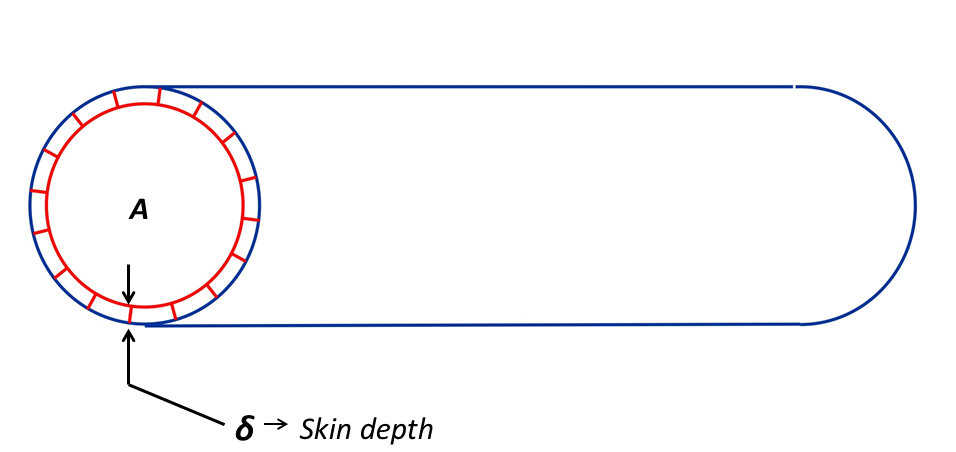
\includegraphics[width=1\linewidth]{\pathtopartone/graphics/skin_depth}
\caption{A conductor}
\end{figure}

The region marked A does not contribute to the flow of the current. So even if we make the conductor hollow, the propagation of the energy along the conductor will not be affected since the skin depth layer remains intact. To have good propagation, the property of the small thin layer should be very good, as any perturbation here will affect the propagation of the electromagnetic wave significantly.

For this reason, if we go to microwave frequency components, where the frequency is very high and the skin depth is very small in microns, the surface has to be perfect as any imperfection will affect the propagation of the electromagnetic wave significantly.
%\begin{figure}[h]
%\centering
%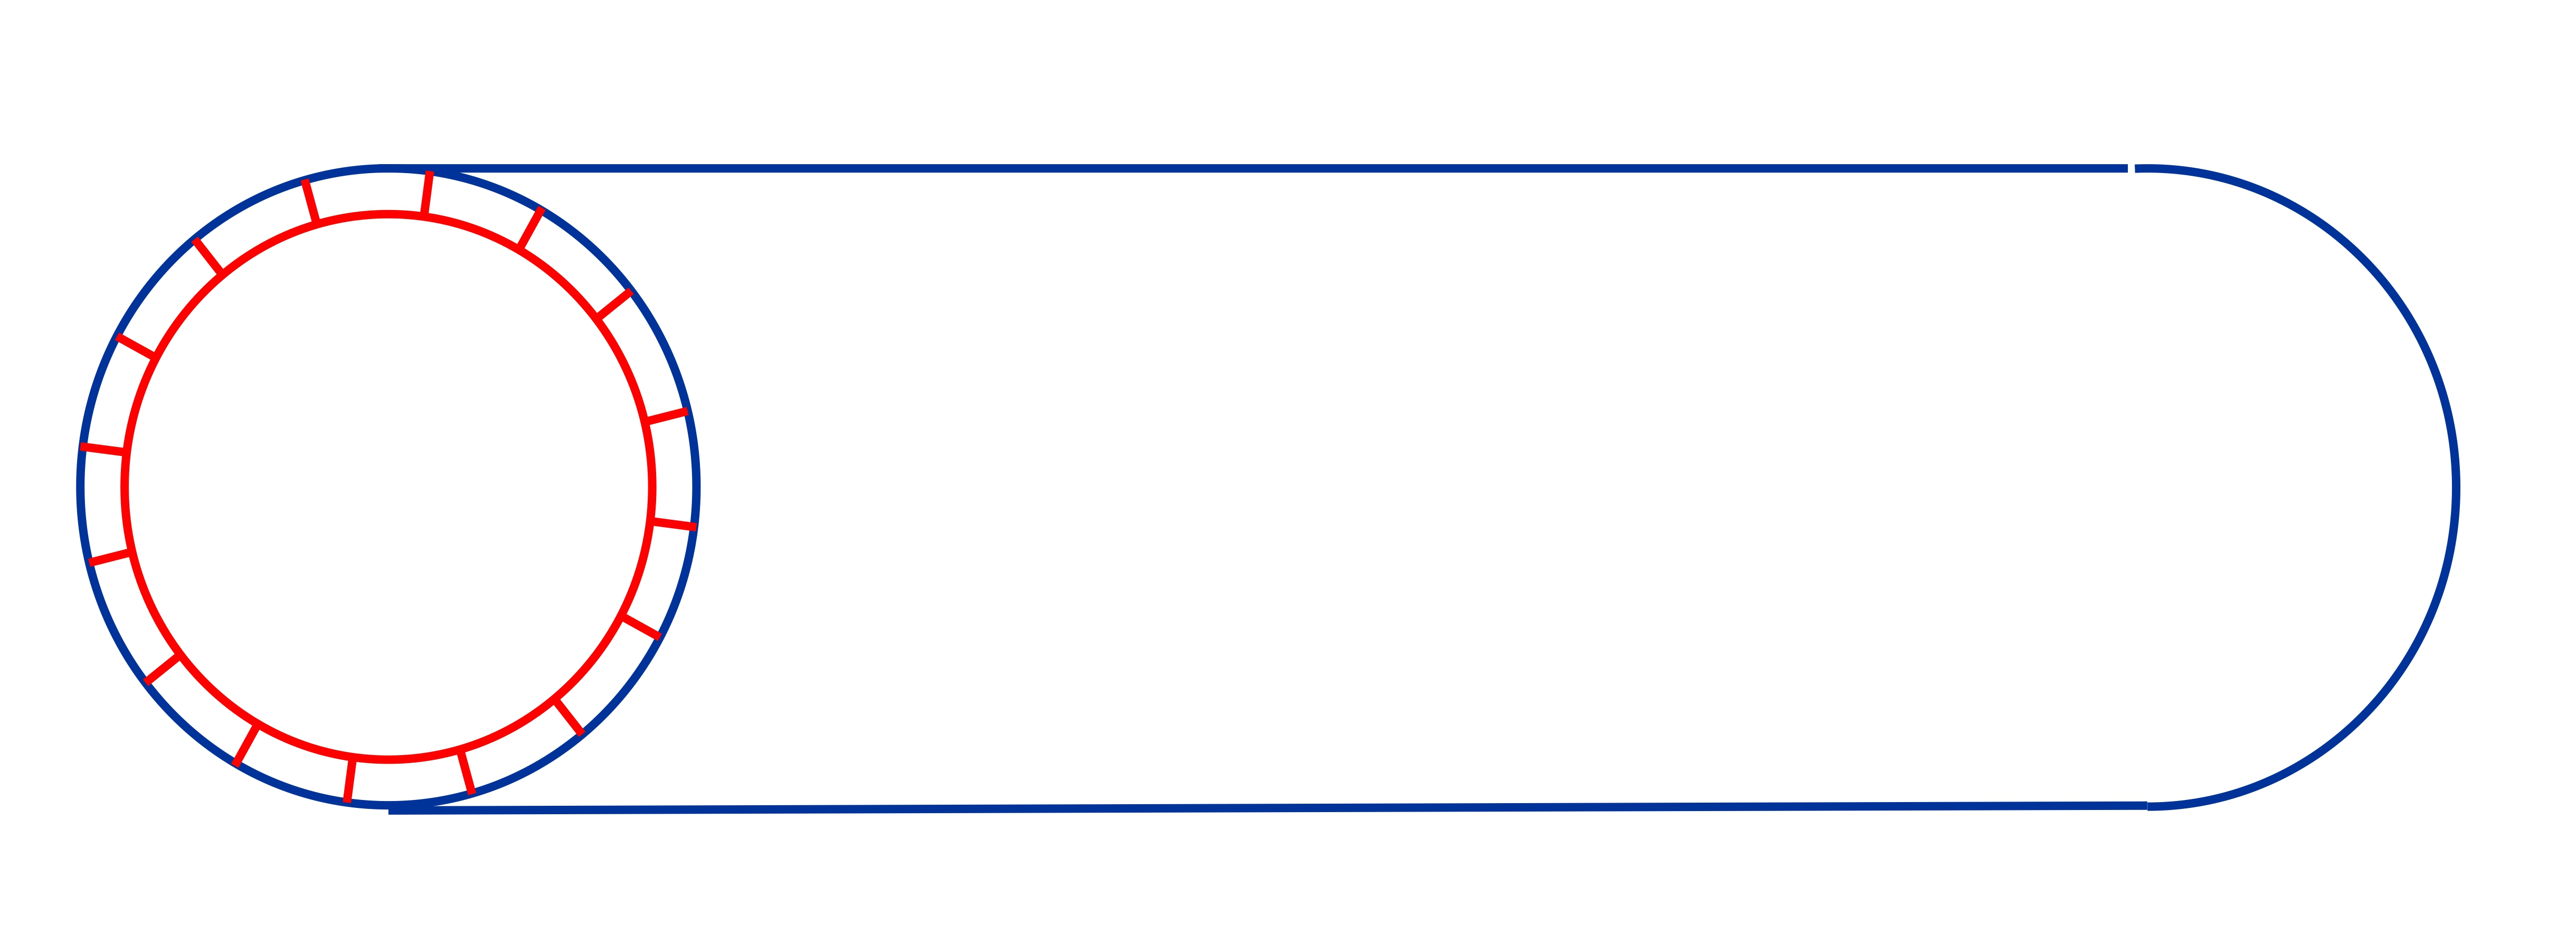
\includegraphics[scale=0.2]{\pathtopartone/graphics/Bello263}
%\caption{An hollow conductor}
%\end{figure}

Let us say we have a conducting medium of finite conductivity as shown above to which we are sending signals along. Considering a certain area of the cross-section for this conductor, at extremely low frequencies, the current is distributed uniformly across the cross-sectional area of this conductor. So we can find out the area of the cross-section and then find out what is the resistance per unit length since the resistivity of the conductor is known.

However, if we increase the frequency, the concept of skin depth starts coming into the picture. The current now gets more and more confined to its surface which means, the area of cross-section over which the current flows reduces. As a result, the resistance of the conductor starts increasing as we go to higher frequencies. So because of the skin depth, the resistance now becomes a function of frequency. For a given conductivity as the frequency increases, the skin depth reduces, and as the skin depth reduces, the area of the cross-section over which the current flows reduces, and because of that, the resistance of the conductor increases.

So what we find out is that the resistance which we treated like the property of the wire is not so when you go to higher frequencies. As the frequency gets higher, the same conductor starts showing higher resistance, and the wave propagation is essentially confined to the surface of the conductor.
For the intrinsic impedance of the medium, $\eta_{c}=\sqrt{\dfrac{j\omega\mu}{\sigma+j\omega\epsilon_{o}\epsilon{r}}}$

And as $\sigma\gg\omega\epsilon_{o}\epsilon_{r}$
\begin{center}
$\eta_{c}\approx\sqrt{\dfrac{j\omega\mu}{\sigma}}=\sqrt{j}\cdot\sqrt{\dfrac{\omega\mu}{\sigma}}$
\end{center}

Recall,
\begin{center}
$\sqrt{j}=\dfrac{1}{\sqrt{2}}+j\dfrac{1}{\sqrt{2}}$
\end{center}

$\eta_{c}$ becomes;
\begin{center}
$\eta_{c}=\sqrt{\dfrac{\omega\mu}{\sigma}}\Bigg\{\dfrac{1}{\sqrt{2}}+j\dfrac{1}{\sqrt{2}}\Bigg\}$
\end{center} 

\begin{center}
$\eta_{c}=\sqrt{\dfrac{\omega\mu}{\sigma}}<45^{o}$ in terms of magnitude and phase.
\end{center}

Therefore, the Electric and Magnetic fields are related to the intrinsic impedance of the medium.

For a Dielectric Medium
\begin{center}
$\dfrac{|E|}{|H|}=\eta,$
\end{center}

So in this case, $\dfrac{|E|}{|H|}=\eta_{c}=\sqrt{\dfrac{\omega\mu}{\sigma}}<45^{o}$

So we see that the electric and magnetic fields are still perpendicular to each other but there is a time lag in the magnetic field compared to the electric field. The ratio $\frac{|E|}{|H|}$ is now dependent on frequency and not only on the medium parameter, as it used to be in the case of the dielectric medium. So when we talk about a good conducting medium, important things happen.

When the wave tries to penetrate, the wave is restricted to a very short distance called the conducting depth. Also, the electric and magnetic fields are not in the time phase anymore, there is a phase difference in time which is 45\textdegree.

So the wave propagation in a dielectric medium and a conducting medium are completely different. In a dielectric medium, the wave can go deep into the medium, and the electric and magnetic fields are in the time phase. The wave amplitude reduction is very small. Whereas in a conducting medium, the wave amplitude drops very rapidly, it can't go deep into the medium, and also, the electric and magnetic fields have a phase difference in time.

If we take a general medium which is a combination of a dielectric and a conductor, then all these relationships are going to be complex as we don't have any approximations. For those media, for which conduction current is comparable to displacement current, we have to do a rigorous analysis. For the two extreme cases i.e. good dielectric and good conductor, this approximation can be made easily and one can understand the wave propagation in a more comprehensible manner than in the general medium.
Now we go into another aspect, \emph{which is, what will be the velocity of the wave as it tries to move in this medium?} Let us take a medium that is a good dielectric and assume the losses are very small, so we can treat the dielectric almost like a lossless dielectric. Then we ask the question \emph{``How is the wave going to propagate in this medium?"} If the medium is lossless, the propagation constant is purely imaginary, and then any field E can be written as:
\begin{center}
$\bar{E}=\bar{E_{o}}e^{-j\beta x}e^{j\omega t}=\bar{E}_{o}e^{j\{\omega t-\beta x\}} $
\end{center}

This represents a wave travelling in a positive direction. Now if we stand on a particular location in space i.e. x is constant and look at the wave which is moving in space, the phase of the wave will vary with respect to time (with $wt$). That is, the phase is linearly increasing as a function of time. However, suppose we hold on to a particular phase point on the wave, say we are holding on to A since the wave is moving, we will move along with the wave with the velocity at which the wave is travelling if we don't want to lose that phase point we are holding on to.
\begin{figure}[h]
\centering
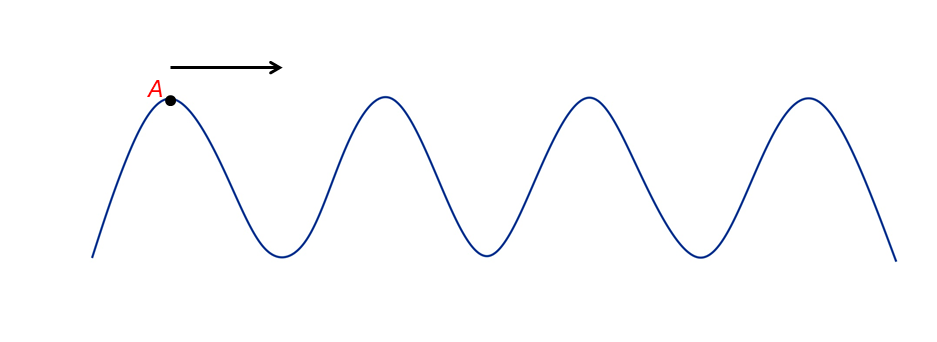
\includegraphics[width=1\linewidth]{\pathtopartone/graphics/constant_phase}
\caption{A wave form}
\end{figure}

So for an observer holding on to A, the phase does not change anymore. Hence, to the observer, the phase appears to be constant as a function of time. So by making the phase of the wave($wt - \beta x$) constant as a function of time, whatever speed the observer needs to move at to keep this phase constant is the velocity of the wave. So basically, we make the phase constant as a function of time to get the velocity of the wave.
\begin{center}
$\omega t-\beta x = constant$
\end{center}

Differentiating, we have
\begin{center}
$\omega-\beta\frac{dx}{dt}=0$
\end{center}

Meanwhile, 
\begin{center}
$\frac{dx}{dt}=velocity=\frac{\omega}{\beta}$
\end{center}

\section{\textbf{Phase Velocity}}
The velocity we calculated from the phase being stationary, is called the \textbf{PHASE VELOCITY} of the wave. That means a constant phase point on the wave is moving with this velocity. This concept of naming the velocity is necessary because we are going to encounter another velocity of the wave with which the energy travels.

However, when we talk about waves moving in some arbitrary direction, this concept of saying that the phase is moving with this velocity comes into play because the energy might move in some other velocity. We call the velocity of this constant phase, the phase velocity $ v_p $.

\begin{center}
$ v_p=\frac{\omega}{\beta} $
\end{center}

For a given frequency in any medium, we find out what its phase constant $\beta  $ is, then $\frac{\omega}{\beta}$ gives a quantity which is the velocity that is called Phase Velocity.

Essentially, the knowledge of propagation constant $(\gamma=\alpha+j\beta)$ is important because that tells the phase of the wave when it travels through the medium.
For a travelling wave, this is very straightforward, we get $ \omega t-\beta x=constant $. However, the concept of phase velocity can be extended to any arbitrary wave propagation. For example, suppose we have two waves that are travelling in opposite directions, which forms a standing wave, we can still define the total phase which is a combination of space and time. By making that quantity stationary as a function of time, we get the expression for the phase velocity of the wave. So the concept is very general, Though for travelling wave it is very simple, and so we easily get its phase velocity as $v_{p} = \frac{\omega}{\beta}.$ We will use this relation often when we go to the propagation of electromagnetic waves.

\section{\textbf{The Case of a Pure Dielectric}}

As we have seen earlier, if we take a dielectric medium, that is a PURE DIELECTRIC($\epsilon_{r}$)

The phase constant will be:

\begin{center}
$\beta=\omega\sqrt{\mu_{o}\epsilon_{o}\epsilon_{r}}$ 
\end{center}

Let's consider free space (i.e. $\epsilon_{r}=1 $), then for free space, $\beta=\omega\sqrt{\mu_{o}\epsilon_{o}}$.
Since phase velocity $v_p=\frac{\omega}{\beta}$, phase velocity in free space will become;

$v_p=\dfrac{\omega}{\omega\sqrt{\mu_{o}\epsilon_{o}}}=\dfrac{1}{\sqrt{\mu_{o}\epsilon_{o}}}=$ 

$\dfrac{1}{\sqrt{4\pi\times 10^{-7}\times \frac{1}{36\pi}\times 10^{-9}}}=3\times 10^{8}m/s.$

At this point, we noticed that the velocity of the wave when it is travelling in free space is the velocity of light in free space. Since light is a transverse electromagnetic wave, it is travelling with a velocity given by the phase velocity, $v_{p} = 3\times 10^{8}m/s$. So any wave, not only light which is a transverse electromagnetic wave travelling in free space, will have a velocity equal to $3\times 10^{8}m/s$. $v_p$ is the velocity in vacuum denoted by c.
We can therefore represent the velocity of the wave in a dielectric medium as;

$v_p=\dfrac{\omega}{\omega\sqrt{\mu_{o}\epsilon_{o}\epsilon_{r}}}=\dfrac{1}{\sqrt{\mu_{o}\epsilon_{o}}}\times \dfrac{1}{\sqrt{\epsilon_{r}}}=\dfrac{c}{\sqrt{\epsilon_{r}}}$

So we see that for $\epsilon_{r}\neq 1$ when an electromagnetic wave travels in a medium, its phase velocity is not exactly equal to  $3\times 10^{8}m/s$ because of $\epsilon_{r}$. If $\epsilon_{r}>1$, then the phase velocity will always be less than $c$ (that is, $3\times 10^{8}m/s$). Where c is the velocity of light in free space.

So the velocity of a wave in any dielectric medium is always less than the velocity in free space. We also know that the refractive index of the medium is defined as the ratio;
\begin{equation}
\textbf{Refractive Index($\eta$)} =	\dfrac{\text{Velocity of light in a vacuum}}{\text{Velocity of light in a medium}}
\end{equation}
Therefore,
\begin{center}
$\dfrac{\text{Velocity of light in a vacuum}}{\text{Velocity of light in a medium}}$	
= $\dfrac{c}{v_{p}}$ = $\sqrt{\epsilon_{r}}$  
\end{center}

So the Refractive index of a lossless medium is given by  $\eta$ = $\sqrt{\epsilon_{r}}$. So whenever we have a medium that is pure dielectric or good dielectric, the refractive index and dielectric constant are related by this relationship. The electromagnetic wave always slows down in a medium compared to a vacuum, when the medium has a dielectric constant greater than 1.
Let us take a look at what happens when we apply the relationship to a conductor;

$\beta=\sqrt{\dfrac{\omega\mu_{o}\sigma}{2}}$  and   $v_p=\dfrac{\omega}{\beta}=\dfrac{\omega}{\sqrt{\frac{\omega\mu_{o}\sigma}{2}}}=\sqrt{\dfrac{2\omega}{\mu_{o}\sigma}}$

So the velocity we had for a dielectric medium $\frac{C}{\sqrt{\epsilon_{r}}}$ was not a function of frequency, sine $\epsilon_{r}$ is not a function of frequency, so $v_p$ is not frequency dependent for dielectric material. i.e. all frequency starts with the same speed in the medium.
However, for a medium which is a conductor $v_p=\sqrt{\frac{2\omega}{\mu_{o}\sigma}}$, even if medium properties are not varying as a function of frequency, $\beta=\sqrt{\frac{\omega\mu_{o}}{2}}$ and $v_p$ are functions of frequency.

This medium is thus called a DISPERSIVE MEDIUM because the velocity is varying as a function of frequency. Hence, all frequencies do not travel at the same speed and because of that, we have a dispersion in the medium, so we have an important contribution to draw.
We got the phase velocity and realize that for a dielectric material, the phase velocity depends on the dielectric constant of the medium, and for $\epsilon_{r} > 1$, the $v_p$ is always less than the phase velocity in vacuum. Though the wave slows down, it is not a dispersive medium since all frequencies travel at the same speed. We find that the refractive index, $\eta$ = $\sqrt{\epsilon_{r}}$.

However, for the conductor, $v_p$ is a function of frequency i.e. the medium becomes a dispersive medium. So a pure dielectric medium is a Non Dispersive medium, and a good conductor is a dispersive medium. This essentially summarizes the propagation of a transverse electromagnetic wave in an unbound medium. Before we proceed further, we have to investigate first the power flow associated with the electromagnetic waves and then treat the more complex analysis of the propagation of Electromagnetic waves in a bound medium or in a medium with interfaces that are dielectric or conducting interfaces.

